% !TeX encoding = UTF-8
% !TeX spellcheck = de_DE
\documentclass[ngerman]{article}

\usepackage{arxivDE}

\usepackage[utf8]{inputenc}
\usepackage[T1]{fontenc}

\usepackage{graphicx}

\usepackage[
	backend=biber,
	style=authoryear,
	citestyle=authoryear,
	hyperref
]{biblatex}
\usepackage{csquotes}
\usepackage[ngerman]{babel}
\usepackage[ngerman=ngerman-x-latest]{hyphsubst}

\usepackage{booktabs}

\usepackage{siunitx}
\sisetup{locale=DE}


\usepackage{hyperref}
\usepackage{url}

\addbibresource{references.bib}
\graphicspath{{figures/}, {images/}}

\title{
    Multimodaler Bedeutungstransfer vom Text zum Bild.\\
    Granulare Bildklassifikation durch Verteilungssemantik.
}

\author{
	Simon Donig \href{https://orcid.org/0000-0002-1741-466X}{
\includegraphics[scale=0.06]{orcid.png}}\\
    Lehrstuhl für Digital Humanities\\
    Universität Passau, Deutschland\\
    \url{simon.donig@uni-passau.de}\\
    \And
    Maria Christoforaki \\
    Lehrstuhl für Data Science\\
    Institut für Informatik\\
    Universität St.Gallen, Schweiz \\
    \url{maria.christoforaki@unisg.ch} \\
    \AND
    Bernhard Bermeitinger \href{https://orcid.org/0000-0002-2524-1850}{
\includegraphics[scale=0.06]{orcid.png}} \\
    Lehrstuhl für Data Science\\
    Institut für Informatik\\
    Universität St.Gallen, Schweiz \\
    \url{bernhard.bermeitinger@unisg.ch} \\
    \And
    Siegfried Handschuh \\
    Lehrstuhl für Data Science\\
    Institut für Informatik\\
    Universität St.Gallen, Schweiz \\
    \url{siegfried.handschuh@unisg.ch} \\
}

\date{Dezember 2019}

\hypersetup{
	pdftitle={Multimodaler Bedeutungstransfer vom Text zum Bild. Granulare Bildklassifikation durch Verteilungssemantik.},
	pdfauthor={Simon Donig, Maria Christoforaki, Bernhard Bermeitinger, Siegfried Handschuh},
	pdfkeywords={deep learning, artificial neural networks, digital humanities, distributional semantics, neoclassicism}
}

\begin{document}

\maketitle

% !TeX encoding = UTF-8
% !TeX spellcheck = de_DE
\section{Einleitend}
In den letzten Jahren hat die Verwendung von Bildklassifizierungsverfahren wie neuronalen Netzwerken auch im Bereich der historischen Bildwissenschaften und der \emph{Heritage Informatics} weite Verbreitung gefunden \parencite{lang_AttestingSimilaritySupportingOrganizationStudy_2018}. Diese Verfahren stehen dabei vor einer Reihe von Herausforderungen, darunter dem Umgang mit den vergleichsweise kleinen Datenmengen sowie zugleich hochdimensionalen Datenräumen in den digitalen Geisteswissenschaften. Meist bilden diese Methoden die Klassifizierung auf einen vergleichsweise flachen Raum ab. Dieser flache Zugang verliert im Bemühen um ontologische Eindeutigkeit eine Reihe von relevanten Dimensionen, darunter taxonomische, mereologische und assoziative Beziehungen zwischen den Klassen beziehungsweise dem nicht formalisierten Kontext. Eine in \parencite{donig_VomBildTextUndWieder_2019a} vorgeschlagene Lösung, diese Beziehungen wieder in den Prozess der Klassifizierung zurückzubringen, ist, sich die größere Ausdruckskraft von textbasierten Modellen zunutze zu machen, um die Fähigkeiten visueller Klassifikatoren zu erweitern. 

Dabei wird ein \mbox{\emph{Convolutional Neural Network} (CNN)} genutzt, dessen Ausgabe im Trainingsprozess, anders als herkömmlich, nicht auf einer Serie flacher Textlabel beruht, sondern auf einer Serie von Vektoren. Diese Vektoren resultieren aus einem \mbox{\emph{Distributional Semantic Model} (DSM)}, welches aus einem Domäne-Textkorpus generiert wird. Ein DSM ist ein multidimensionaler Vektorraum, in dem Wörter als Vektoren abgebildet werden \parencite{lenci_DistributionalModelsWordMeaning_2018a}.

Das durchgeführte Experiment beruht auf der Kollation von zwei Korpora: Einem textbasierten und einem visuellen. Mit dem Textkorpus wird zunächst ein DSM erzeugt und diesem dann eine Auswahlliste von Zielwörter zugeführt (die funktional den Annotationslabeln der Bilder entspricht). Als Ergebnis erhalten wir Vektoren, die mit diesen Wörtern korrespondieren und mit denen die Bilder annotiert werden. Mit diesen Vektorannotationen wird ein neuronales Netzwerk trainiert, das anschließend dem Klassifikator unbekanntes Bildmaterial identifizieren soll. Als Ergebnis dieses Klassifikationsprozesses erhalten wir einen Vektor, der mithilfe des DSMs in natürlichsprachige Wörter zurückgewandelt wird. Da wir nach reicheren Repräsentationen im Zuge dieses Vorgangs suchen, wählen wir die fünf nächsten Nachbarn aus (\mbox{\emph{Top-5 Nearest Neighbors}}). Als Ähnlichkeitsmaß legen wir die Kosinusähnlichkeit zwischen dem vorhergesagtem Vektor und jenem Vektor zugrunde, der dem ursprünglich dem Bild von uns zugewiesenen Textlabel entspricht. Wir gehen davon aus, dass ein Bild korrekt klassifiziert wurde, wenn das Goldlabel unter diesen Top-5 erscheint.

Darüber hinaus vergleichen wir die Ergebnisse des vorgeschlagenen Klassifizierungsverfahrens mit einem herkömmlichen Verfahren auf der Grundlage flacher Label unter Verwendung desselben CNNs, das für das Vektor-Experiment genutzt wurde. Wir können zeigen, dass das Vektor-Verfahren (bezogen auf die Metriken) ebenso effizient und in einigen Aspekten sogar besser ist.

\section{Aufbau des Experiments}
Das Experiment beruht auf je einem Bild- und Textkorpus aus dem Bereich Sachkulturforschung mit einem Fokus auf klassizistische Artefakte.

\subsection{Textkorpus}
Das Textkorpus besteht aus 44 Quellen, die unter einer freien, permissiven Lizenz verfügbar sind, und umfasst englischsprachige Fachpublikationen zu Mobiliar und Raumkunst, die von  der Jahrhundertwende bis zur Mitte des 20.~Jahrhunderts erschienen sind. Das Textkorpus wurde in mehreren Schritten gereinigt und aufbereitet: Zum einen wurden Standard-NLP-Verfahren angewandt, darunter Tokenisierung, Satz- und Worttrennung, die Normalisierung von Zahlenwerten und die Erkennung von benannten Entitäten (\emph{Named Entity Recognition, NER}). Da wir retrodigitalisiertes Material aus verschiedenen Quellen nutzen, implementieren wir manuelle Korrekturen für die häufigsten der vorkommenden Fehler (etwa Ligaturen wie \texttt{II}, die als \texttt{U} durch das OCR-Verfahren fehlinterpretiert werden). Eine weitere Ebene der Vorverarbeitung besteht aus inhaltsbezogenen Augmentierungen. Insbesondere normalisieren wir zusammengesetzte Wörter und Synonyme gemäß einer spezifizierten Liste, die anhand einer Ontologie, der \emph{Neoclassica-Ontologie} \parencite{donig_NeoclassicaMultilingualDomainOntology_2016} zusammengestellt sind. Dies resultiert in einem Korpus von insgesamt \num{3067237} Wörtern aus \num{107518} Wortgrundformen.
Das DSM wird von uns mithilfe des \emph{Indra}-Frameworks \parencite{sales_IndraWordEmbeddingSemanticRelatedness_2018a} sowie \emph{Gensim} \parencite{rehurek_lrec} erzeugt\footnote{Die Erzeugung erfolgt mit einer Vektorgröße von 50, einer Worfenstergröße von 10 und einer minimalen Wortzahl von fünf erzeugt. Als \emph{Word2Vec}-Modell kommt \emph{Skipgram} \parencite{mikolov_EfficientEstimationWordRepresentationsVector_2013} mit \emph{Negative Sampling} zum Einsatz.}.


\subsection{Bildkorpus}
Das Bildkorpus besteht aus \num{1231} Ansichten klassizistischer Möbel in deren Gesamtheit, die permissiv lizenziert sind\footnote{Das Korpus wurde aus den Sammlungen des Metropolitan~Museum (New~York), des Victoria~\&~Albert~Museum (London), der Wallace~Collection (London) sowie mehreren zeitgenössischen Musterbüchern zusammengestellt.} und die sowohl historisches Bildmaterial als auch Fotos aus der modernen Bestandsdokumentation umfassen. Es repräsentiert 28 Klassen.


\subsection{Kombiniertes Korpus}
Da es sich um ein \emph{Proof-of-Concept}-Experiment handelt, kommt zum Zweck des \emph{Rapid Prototypings} ein an die VGG-Architektur \parencite{krizhevsky_ImageNetClassificationDeepConvolutionalNeural_2012a} angelehntes, \enquote{simples} neuronales Netzwerk zum Einsatz\footnote{Das Netzwerk besteht aus drei Convolutional-Blöcken mit jeweils zwei Convolutional-Layer mit \numlist{32;64;64} Filter der Größe $ 3 \times 3 $. Nach jedem Block folgt ein Maximum-Pooling-Layer der Größe $ 2 \times 2 $, sowie ein Dropout-Layer mit einer Dropoutwahrscheinlichkeit von \num{0.25}. Ein Fully-Connected-Block, bestehend aus zwei Fully-Connected-Layers mit jeweils 256 Knoten, steht im Anschluss sowie nochmals ein Dropout-Layer mit \num{0.5} Dropoutwahrscheinlichkeit. Jeder Convolutional- und Fully-Connected-Layer bis dahin wurde zufällig initialisiert und benutzt \emph{ReLU} als Aktivierungsfunktion. Der letzte Layer ist ein Fully-Connected-Layer mit 50 Ausgabeknoten und benutzt eine lineare Aktivierungsfunktion. Es ist in den beiden Frameworks \emph{Keras} (\url{https://keras.io}) und \emph{TensorFlow} (\url{https://tensorflow.org}) implementiert. Beim Training wird der durchschnittliche absolute Fehler durch die Optimierungsfunktion \emph{RMSprop} minimiert.}.
Die Unabhängigkeit der Trainings- und Evalutationsbeispiele wird durch eine \mbox{5-fache} Kreuzvalidierung auf \SI{80}{\percent} des Korpus garantiert, wovon wiederum \SI{80}{\percent} für das Training und \SI{20}{\percent} für das Testen benutzt werden. Die übrigen \SI{20}{\percent} werden als Evaluationsmenge behandelt. Die reportierten Ergebnisse basieren auf diesen, dem Klassifikator unbekannten \SI{20}{\percent}. 

Da durch Sammlungspraxis der Gedächtnisinstitutionen (Sammelwürdigkeit, geografischer Schwerpunkt) und Zugänglichkeit des Materials (Lizenzierung und Grad der Sammlungsdigitalisierung) die Verteilung der Artefakte nach Klassen unbalanciert ist (Abb.~\ref{fig:class_distribution}), sind die Klassengewichte dementsprechend angepasst (seltene Klassen werden höher gewichtet als häufig vorkommende Klassen \parencite[S.~27]{johnson_SurveyDeepLearningClassImbalance_2019}). Um eine Situation zu vermeiden, in der ein \emph{Machine-Learning}-Modell derart an die Trainingsdaten angepasst wird, dass es darin scheitert auf anderen, aber trotzdem ähnlichen Daten, zu generalisieren, wird die übliche \emph{Early-Stopping}-Methode verwendet. 

\begin{figure}
	\centering
	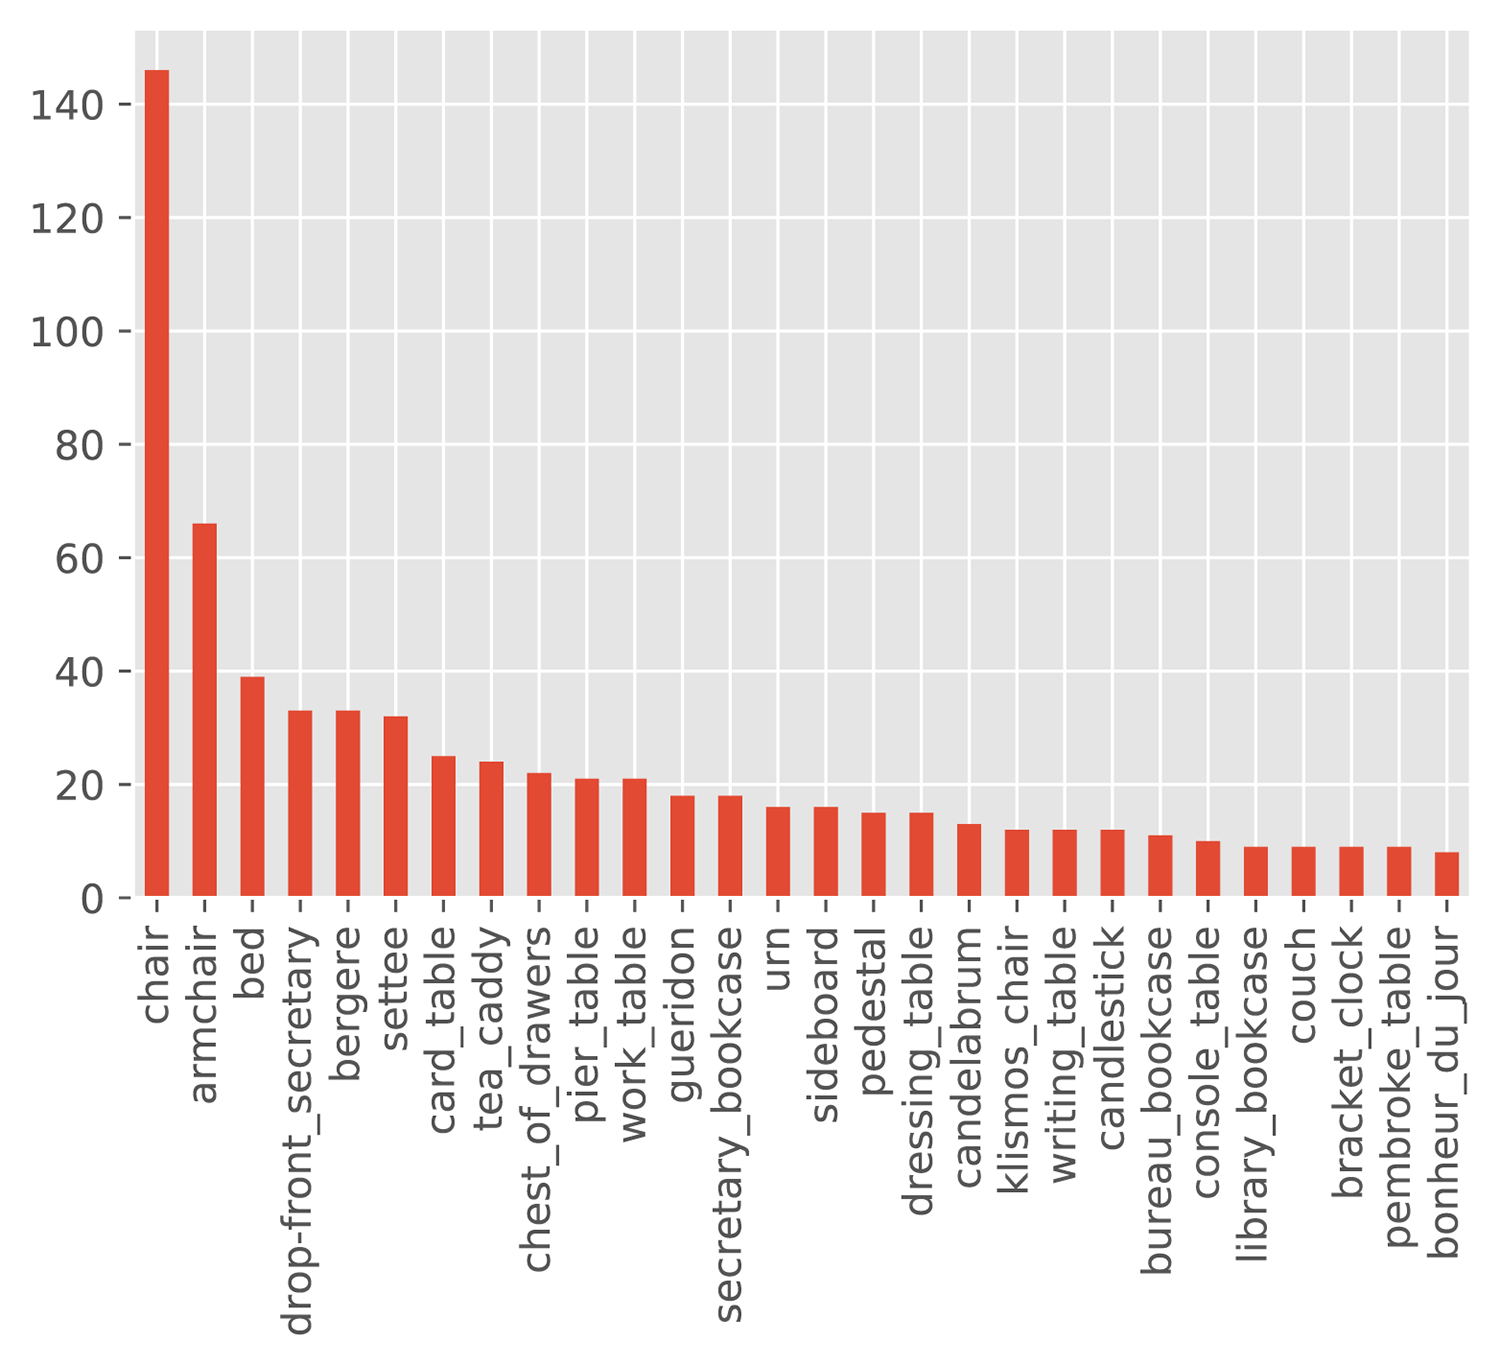
\includegraphics[height=.5\textheight]{class_distribution.png}
	\caption{Verteilung der Klassen im Bildkorpus.}
	\label{fig:class_distribution}
\end{figure}

\section{Ergebnisse}
Die \mbox{Top-5-Richtig-Positiv-Rate} (\emph{true-positive}) beträgt \num{0.59}. Das bedeutet, dass das Goldlabel in \SI{59}{\percent} der Fälle unter den fünf nächsten Nachbarn erscheint.

Das mathematische Qualitätskriterium gibt für sich genommen jedoch nur einen Teil des Gesamtbilds wieder. Wir führen deshalb zugleich eine qualitative Analyse der Ergebnisse in der Evalutionsteilmenge durch.

Eine Reihe von richtig-positiven Ergebnissen zeigen, dass die Klassifizierung keinesfalls zufällig erfolgt, sondern dass die \mbox{Top-5-Begriffe} tatsächlich jeweils denselben semantischen Nachbarschaften entstammen. Sie drücken eine Reihe von Beziehungen taxonomischer und assoziativer Natur aus.
Beispielsweise wird der \mbox{Roentgen-Schreibtisch} aus dem Bestand des V\&A in Abb.~\ref{fig:classification_same_object_1} mit Labeln (in der Reihenfolge) von \texttt{dressing\_table}, \texttt{writing\_table} und \texttt{work\_table} assoziiert (Ankleidetisch, Schreibtisch, Nähtisch). Diese Trias ist schon deshalb sinnhaltig, weil viele dieser Artefakte multifunktional waren und mehrere dieser Funktionen erfüllten. Daneben ähneln auch jene Artefakte, die dezidiert nur einem einzigen Zweck dienten, konstruktiv den jeweils anderen Möbeltypen. Die Nähe der drei Konzepte entsteht also sowohl auf semantischer Ebene (Nähe der Wörter im DSM, die wiederum das Produkt lebensweltlicher Nähe ist), als auch auf einer visuellen Ebene im CNN (visuelle Formähnlichkeit). Ein weiteres Bild desselben Objekts (Abb.~\ref{fig:classification_same_object_2}) zeigt einerseits, dass die Methode in sich konsistent ist (die Top-4 sind identisch, obwohl eine andere Perspektive vorliegt) und andererseits, dass auch die visuellen Merkmale innerhalb des CNNs eine Auswirkung auf den Klassifizierungsprozess haben. Da Schreibschränke (\emph{secrétaires à abbatants}) häufig frontal, hochaufrecht und mit einer geöffneten Schreibklappe oder -schublade abgebildet werden, scheint deren Vorkommen im Bild eine Klassifizierung als Sekretär ausgelöst zu haben. Im ersten Bild könnte dagegen die Anwesenheit von Schubladen (\emph{drawers}) zu einer Klassifizierung als Kommode geführt haben, die naheliegenderweise auf semantischer Ebene mit Schubladen assoziiert ist.

\begin{figure}
	\centering
	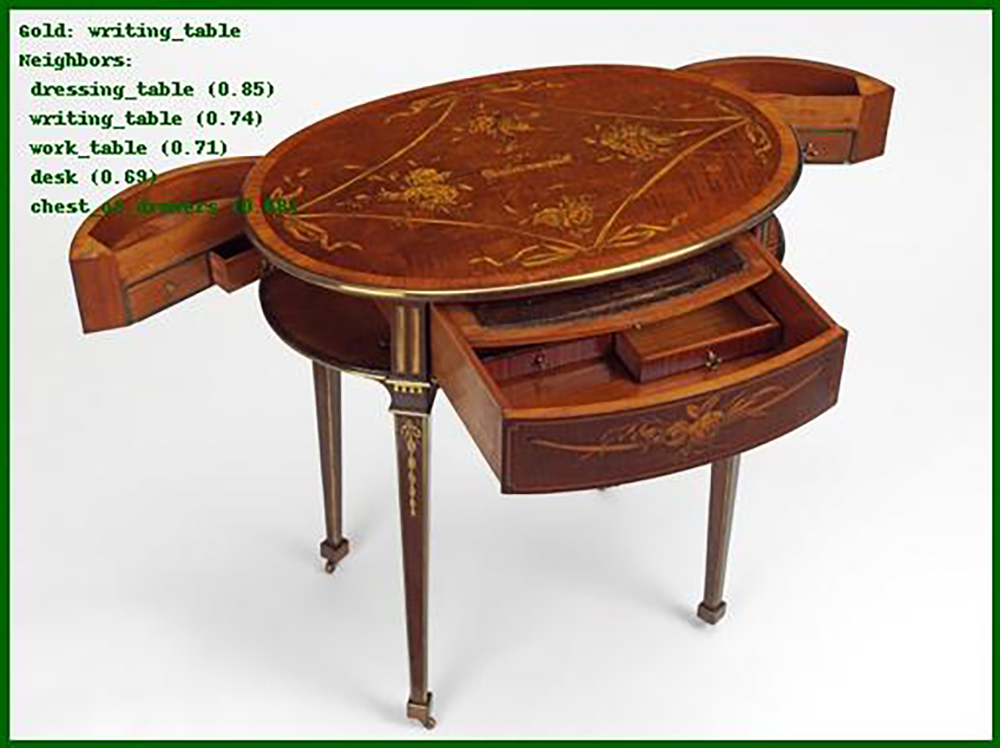
\includegraphics[height=.4\textheight]{classification_same_object_1.png}
	\caption{Abweichungen bei der Klassifizierung desselben Objekts \parencite{victoriaalbertmuseum_WritingTableNeuwiedWorkshopDavid_2019}.}
	\label{fig:classification_same_object_1}
\end{figure}

\begin{figure}
	\centering
	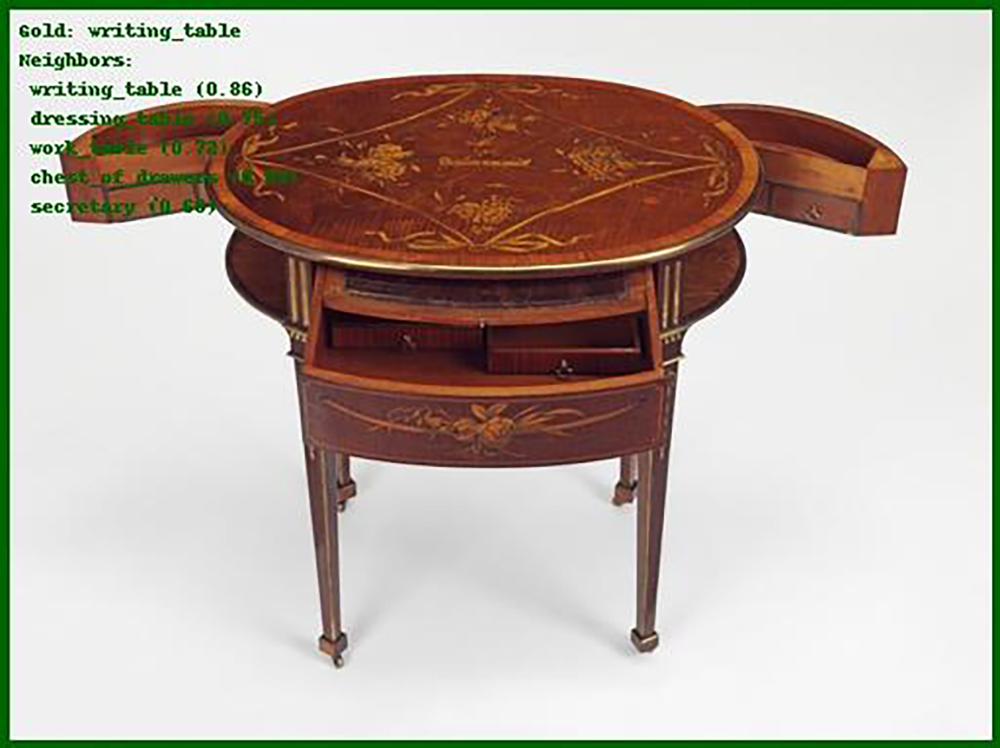
\includegraphics[height=.4\textheight]{classification_same_object_2.png}
	\caption{Abweichungen bei der Klassifizierung desselben Objekts \parencite{victoriaalbertmuseum_WritingTableNeuwiedWorkshopDavid_2019}.}
	\label{fig:classification_same_object_2}
\end{figure}

Während die Label in den bisher betrachteten Fällen die taxonomischen Beziehungen reflektieren und alle den aus der Ontologie abgeleiteten Zielwörtern entstammen, zeigt Abb.~\ref{fig:medici_vase}, dass das Verfahren auch aus sich selbst, rein datenzentriert Label generieren kann. Die abgebildete Kratervase wurde manuell als Urne (\emph{urn}) annotiert. Die \mbox{Top-2-Wörter} reflektieren demnach auch taxonomischen Beziehungen (\mbox{\enquote{urn}}, \mbox{\enquote{vase}}). Die anderen Konzepte spiegeln dagegen assoziative Beziehungen wider. Das Label \texttt{bell} ist ein Artefakt des Reinigungsprozesses, da im Korpus Wörter wie \mbox{\enquote{bell-shaped}} oder \mbox{\enquote{bell-crater}} (mit und ohne Bindestrich) existieren, um diese Art von Artefakten zu beschreiben. \enquote{Ovoid} bezieht sich demgegenüber wohl auf die Eierstabdekoration des oberen Wulstes, die oft mit diesem Adjektiv beschrieben wird. Diese Ornamentik scheint zugleich die Assoziation zur Rosette (\emph{Patera}) mitbedingt zu haben. Auf diese Weise erscheint das Zielwort \texttt{patera\_element} unter den \mbox{Top-5}, obwohl im Bildkorpus ausschließlich ganze Artefakte, nicht aber deren Dekor annotiert wurden. 

\begin{figure}
	\centering
	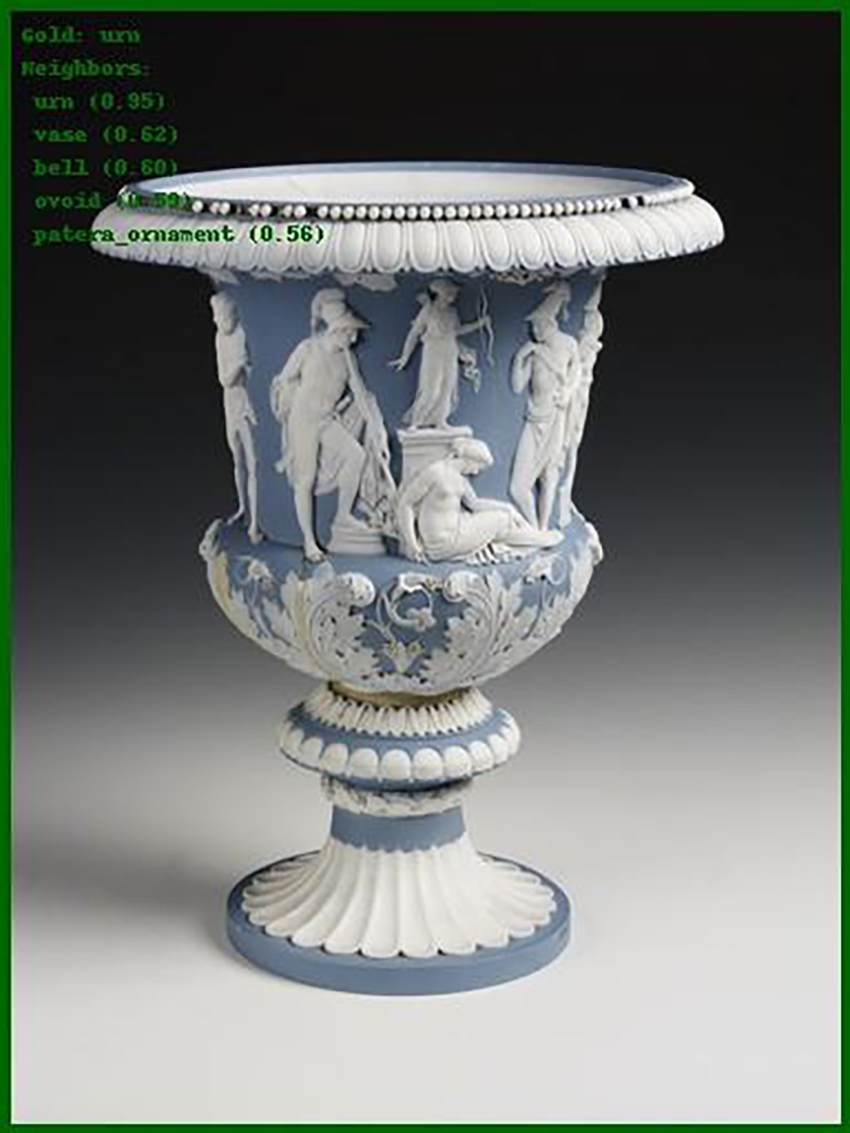
\includegraphics[height=.6\textheight]{medici_vase.png}
	\caption{Eine Sèvres-Kopie der Medici-Vase stößt die Klassifizierung mit assoziativen Labeln an. \parencite{victoriaalbertmuseum_VaseSevresCopyMediciVase_2019}}
	\label{fig:medici_vase}
\end{figure}

Nicht auszuschließen ist hier zudem ein Effekt des visuellen Klassifikators, wie auch Abb.~\ref{fig:misclassification} zeigt. Die Fehlklassifikation des Objekts, eines Nähtischchens, führte zu konsistenten Zuschreibungen im Bereich der Sitz- und Liegemöbel. Betrachtet man die äußere Form des Artefakts auf einer abstrakteren Ebene, kann man eine visuelle Nähe zu z.~B.~einem \emph{(Double-) Camel-back Sofa} durchaus nachvollziehen.

\begin{figure}
	\centering
	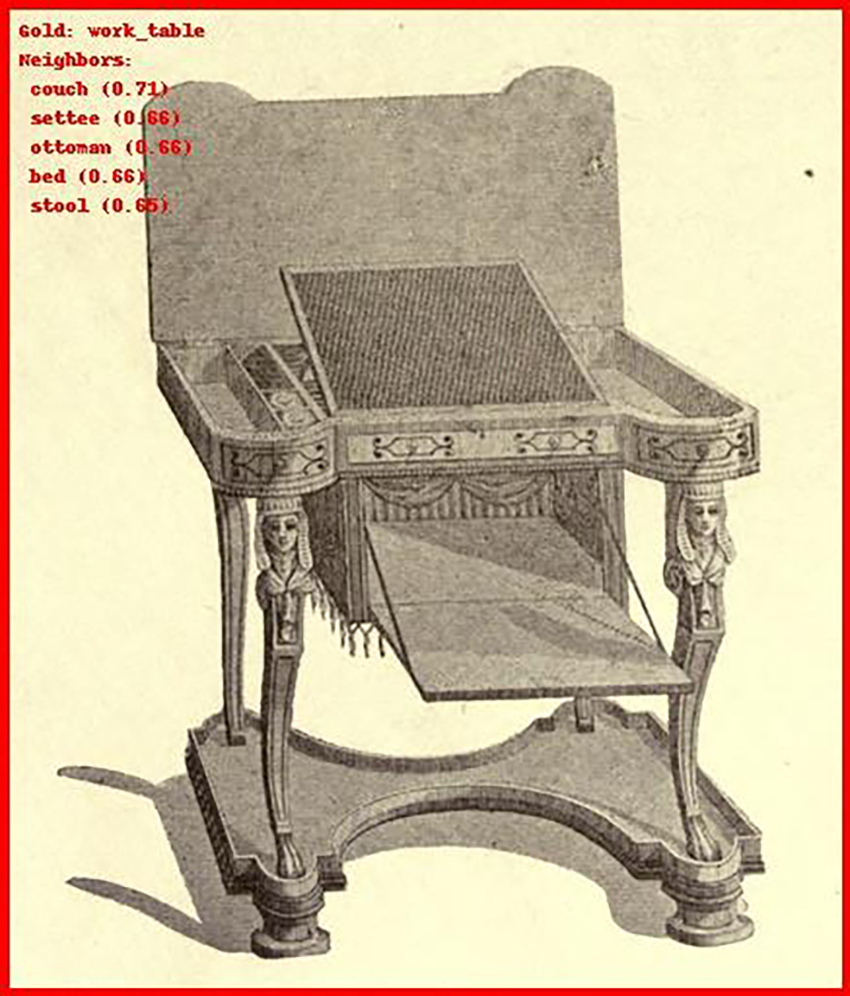
\includegraphics[height=.6\textheight]{misclassification.png}
	\caption{Fehlklassifikation eines Nähtischs in ein Wortumfeld aus der Sitzmöbel-Hierarchie. \parencite[S.~88]{sheraton_FurnitureDesignsThomasSheraton_1910}}
	\label{fig:misclassification}
\end{figure}


\section{Vergleich zu einem herkömmlichen CNN}

Um die Unterschiede zwischen beiden Zugängen besser abschätzen zu können, führen wir weiter in Vergleichsexperiment durch, bei dem dasselbe CNN\footnote{Das verwendete CNN ist identisch mit dem im Vektor-Experiment verwendeten Netzwerk, mit Ausnahme des letzten Layers, der aufgrund der Labelklassifikation nun 28 statt 50 Ausgaben besitzt und die Aktivierungsfunktion \emph{Softmax} statt einer linearen.} wie im vektorbasierten Verfahren für eine herkömmliche Klassifizierung mit flachen Labeln herangezogen wird.

Um die Unterschiede der beiden Zugänge (herkömmliche Klassifizierung mit flachen Labeln/vektorbasiertes Verfahren) besser abschätzen zu können, stellen wir im Folgenden einen Vergleich zentraler Metriken für beide Zugänge vor.

\begin{table}
    \centering
    \begin{tabular}{lrr}
    	\toprule
    	Metrik                    &     Vektor & Flache Label \\ \midrule
    	Top-1-Treffergenauigkeit  & \num{0.50} &   \num{0.40} \\
    	Top-1-Genauigkeit         & \num{0.32} &   \num{0.29} \\
    	Top-1-Trefferquote        & \num{0.25} &   \num{0.26} \\
    	Top-1-F1-Maß              & \num{0.26} &   \num{0.25} \\ \midrule
    	Top-5-Sensitivität        & \num{0.59} &   \num{0.73} \\
    	Top-5-Falsch-Positiv-Rate & \num{0.41} &   \num{0.27} \\
         \bottomrule
    \end{tabular}
    \caption{Vergleich zentraler Metriken beider Zugänge.}
    \label{tab:results}
\end{table}

Wie in Tabelle~\ref{tab:results} ersichtlich\footnote{Die englischen Begriffe für bessere Verständlichkeit: Treffergenauigkeit (\emph{Accuracy}), Genauigkeit (\emph{Precision}), Trefferquote (\emph{Recall}), Sensitivität (\emph{True-Positive Rate})}, ist nicht nur die \mbox{Top-1-Treffergenauigkeit} im Fall der Klassifizierung mit Vektoren besser, sondern es sind auch die übrigen Metriken vergleichbar gut. Durch den hier vorgeschlagenen Zugang wird also nicht nur die Treffergenauigkeit verbessert, sondern er liefert zugleich eine reichhaltigere Beschreibung des Bildes.


\section{Schlussfolgerungen und Ausblick}
In dem hier vorgeschlagenen Beitrag stellen wir ein neues, multimodales Verfahren für die Klassifikation von Bildinhalten vor, das auf der Kombination von NLP-Methoden mit Bildklassifizierungsverfahren beruht. Ziel ist, Objekte nicht alleine nach einem Schema flacher Label, sondern in einer kontextgerechteren Weise zu klassifizieren, wobei dieser Kontext von einschlägigen historischen Domänepublikationen gebildet wird. Dieses Klassifizierungsverfahren bietet einen Zugang zur multidimensionalen Einbettung der Artefakte in die Lebenswelt und deren sprachlicher Widerspiegelung. Dieser Umstand ist von besonderem Nutzen um multifunktionale Objekte zu klassifizieren, ohne dabei auf mehrere Klassifikatoren und einen komplexen Annotationsprozess mit mehreren Labeln zurückgreifen zu müssen. Die Ergebnisse sind ermutigend. Auch mit einem sehr einfachen CNN erreichen wir eine Treffergenauigkeit von \num{0.59}. Als nächsten Schritt möchten wir mit einem komplexeren CNN und einem ausgeweiteten Bildkorpus trainieren (um bekannte Probleme wie \emph{Overfitting} zu reduzieren). Das Vergleichsexperiment mit einem herkömmlichen, auf flachen Labeln beruhenden Zugang zeigt, dass unter Effizienzgesichtspunkten, d.~h.~im direkten Vergleich der Metriken, unser Verfahren nicht nur vergleichbare Resultate liefert, sondern zugleich auch in einer reichhaltigeren Beschreibung des Bildes resultiert.

Wir werden weiter daran arbeiten, besser zu verstehen, wie ein bestimmtes Textkorpus sich in den Labeln widerspiegelt, die das DSM automatisch zuweist und die nicht Teil der Liste der Zielwörter sind. Ein besseres Verständnis dieser Prozesse scheint insbesondere im Hinblick auf die relativ überschaubaren Textkorpora relevant, die in den Geisteswissenschaften zu spezifischen Themenkomplexen kollationiert werden können. Nicht zuletzt werden wir aus diesem Grund die Nutzung von Thesauri und Wörterbüchern in Betracht ziehen, um Synonymlisten für Zielwörter zu erstellen. In ähnlicher Weise ziehen wir in Betracht, benannte Entitäten zu URIs zusammenzufassen. Das würde uns erlauben spezifische Entitäten (z.~B.~Werkstätten, Ebenisten und Eigentümer) mit bestimmten Objekten zu assoziieren.

Wir denken, dass dabei der multimodale Zugriff einen besonders effizienten Zugang zu geistes- und kulturwissenschaftlichen Korpora bietet, die, verglichen mit den Korpora anderer Disziplinen in den Natur- und Sozialwissenschaften, klein und Domäne-restringiert sind.


\printbibliography

\end{document}
